
\section{Brouwer\trDegree}
\label{sec:brouwer-degree}

\hzsync{lemma}{6}
\hzsync{proposition}{7}
\hzsync{equation}{49}

下面我们将描述第 2 章中所使用的所谓\trBrouwer\trDegree{}或\trMapping\trDegree。它为非线性方程
\begin{equation*}
f(x)=y
\end{equation*}
关于 $x$ 的可解性提供了一个定性判据。该\trDegree{}是一个整数，「代数地计数」解的个数。更精确地说，我们考虑 $\R^n$ 中的开有界集 $U$ 与连续\trMapping{} $f:\bar{U}\to\R^n$。给定 $y\in\R^n$，三元组 $(f,\,U,\,y)$ 称为\textbf{容许的}（admissible），若 $y\notin f(\partial U)$。我们的目标是为每个容许三元组关联一个整数，记作 $d(f,\,U,\,y)$，使得赋值
\begin{equation*}
(f,\,U,\,y)\longmapsto d(f,\,U,\,y)
\end{equation*}
满足以下公理所表述的若干自然性质。

\begin{axiom}[\trSolutionProperty]\label{ax:solution-property}
假设 $(f,\,U,\,y)$ 是容许的。若 $d(f,\,U,\,y)\neq 0$，则方程 $f(x)=y$ 在 $U$ 中存在解 $x$。
\end{axiom}

方程 $f(x)=y$ 与 $f(x)-y=0$ 具有相同的解 $x$，因此我们要求

\begin{axiom}[\trNaturality]\label{ax:naturality}
若 $(f,\,U,\,y)$ 是容许的，则
$d(f,\,U,\,y)=d(f-y,\,U,\,0)$。
\end{axiom}

假设 $(f,\,U,\,y)$ 是容许的且 $V\subset U$ 是一个包含全部解的开集，即 $(f|_{U})^{-1}(y)\subset V$。则 $(f,\,V,\,y)$ 也是容许的且具有相同的解，因此我们提出：

\begin{axiom}[\trExcision]\label{ax:excision}
若 $(f,\,U,\,y)$ 是容许的且开集 $V\subset U$ 满足 $f^{-1}(y)\subset V$，则
$d(f,\,U,\,y)=d(f,\,V,\,y)$。
\end{axiom}

我们希望该\trDegree{}「计数」解的个数，因此要求一个可加性质：

\begin{axiom}[\trAdditivity]\label{ax:additivity}
假设 $(f,\,U,\,y)$ 与 $(f,\,V,\,y)$ 是容许的且 $\bar{U}\cap\bar{V}=\emptyset$。则（显然 $(f,\,U\cup V,\,y)$ 也是容许的）
$d(f,\,U\cup V,\,y)=d(f,\,U,\,y)+d(f,\,V,\,y)$。
\end{axiom}

下一条公理是最重要的，对应用至关重要。我们希望解判据在扰动下保持稳定，因此要求 $d$ 在连续形变下不变：

\begin{axiom}[\trHomotopy\trInvariance]\label{ax:homotopy-invariance}
设 $t\mapsto (f_t,\,U,\,y)$，$0\leq t\leq 1$ 是一个容许形变，即 $f:[0,\,1]\times\bar{U}\to\R^n$ 连续且对每个 $0\leq t\leq 1$，$(f_t,\,U,\,y)$ 是容许的。则
$d(f_0,\,U,\,y)=d(f_1,\,U,\,y)$。
\end{axiom}

最后，我们用一个简单的模型方程进行规范化。

\begin{axiom}[\trNormalization]\label{ax:normalization}
$d(\mathrm{Id},\,B_1^n(0),\,0)=1$，
其中 $B_1^n(0)$ 是 $\R^n$ 中以原点 $0$ 为心的开单位球。
\end{axiom}

暂时假设满足这些公理的 $d$ 存在。我们将证明这些公理唯一地确定了 $d$。它被称为\trBrouwer\trDegree{}或\trMapping\trDegree。

首先假设 $U$ 是开集且 $0\notin\bar{U}$。则 $(\mathrm{Id},\,U,\,0)$ 是容许的。由于在 $U$ 中 $\mathrm{Id}(x)=0$ 无解，根据公理 1 我们得出 $d(\mathrm{Id},\,U,\,0)=0$。接下来我们考虑线性映射 $f=T\in\mathrm{Gl}(\R^n)$。

\begin{lemma}\label{lem:brouwer-degree-linear}
假设 $U$ 是 $0$ 的一个有界开邻域且 $T\in\mathrm{Gl}(\R^n)$。则
$d(T,\,U,\,0)=\operatorname{sign}\det T$。
\end{lemma}

\begin{proof}
回忆 $\mathrm{Gl}(\R^n)=G^{+}\cup G^{-}$，其中 $G^{\pm}=\{T\in\mathrm{Gl}(\R^n)\mid \pm\det T>0\}$；$G^{+}$ 与 $G^{-}$ 是\trPathConnected{}的。定义 $\vartheta_{\pm 1}\in\mathrm{Gl}(\R^n)$ 为
\[\vartheta_{\pm 1}=\operatorname{diag}(\pm 1,\,1,\,\ldots,\,1)\,.\]
于是 $\vartheta_{+}\in G^{+}$ 且 $\vartheta_{-}\in G^{-}$。令 $\varepsilon=\operatorname{sign}\det T$\footnote{原书印作「$\varepsilon=\operatorname{sig}\det T$」，其「sig」疑为「sign」漏一「n」之误，此处径改。——译者注} 并在 $G_{\varepsilon}$ 中选取一条连接 $T_0=\vartheta_{\varepsilon}$ 与 $T_1=T$ 的连续道路 $t\mapsto T_t$。则 $t\mapsto(T_t,\,U,\,0)$ 是一个容许形变，由公理 5 我们得到
\[d(\vartheta_{\varepsilon},\,U,\,0)=d(T,\,U,\,0)\,.\]
由于 $0$ 是唯一的解，两次应用\trExcision{}公理我们求得
\[d(T,\,U,\,0)=d(\vartheta_{\varepsilon},\,U,\,0)=d(\vartheta_{\varepsilon},\,B_1^n(0),\,0)\,.\]
若 $\varepsilon=1$，我们运用公理 6 求得
\[d(T,\,U,\,0)=d(\mathrm{Id},\,B_1^n(0),\,0)=1=\operatorname{sign}\det T\,.\]
为了处理 $\varepsilon=-1$ 的情形，对每个 $0\leq\tau\leq 1$ 定义 $\varphi_{\tau}:[-1,\,1]\to\R$ 为 $\varphi_{\tau}(t)=|t|-\tfrac{1}{2}+\tau$，并引入 $f_{\tau}:[-1,\,1]\times B_1^{n-1}(0)\to\R^n$ 为
\[f_{\tau}(x_1,\,\ldots,\,x_n)=(\varphi_{\tau}(x_1),\,x_2,\,\ldots,\,x_n)\,.\]
则 $(f_{\tau},\,(-1,\,1)\times B_1^{n-1}(0),\,0)$ 是一个容许\trHomotopy。若 $\tau=1$，方程 $f_1(x)=0$ 在相关的开集中无解。因此由公理 5，
\[d(f_{\tau},\,(-1,\,1)\times B_1^{n-1},\,0)=0\,,\]
对每个 $\tau\in[0,\,1]$ 成立。若 $\tau=0$，则方程 $|x_1|-\tfrac{1}{2}=0$，$x_j=0$（$2\leq j\leq n$）恰好有两个解：
\[x^{-}=\Bigl(-\frac{1}{2},\,0,\,0,\,\ldots,\,0\Bigr)\,,\qquad x^{+}=\Bigl(\frac{1}{2},\,0,\,\ldots,\,0\Bigr)\,,\]
其中 $x^{-}\in V^{-}:=(-\tfrac{3}{4},\,-\tfrac{1}{4})\times B_1^{n-1}$ 且 $x^{+}\in V^{+}:=(\tfrac{1}{4},\,\tfrac{3}{4})\times B_1^{n-1}$。因此，由\trExcision{}与\trAdditivity{}我们得到
\[0=d(f_0,\,V^{-},\,0)+d(f_0,\,V^{+},\,0)\,.\]
对 $x\in\bar{V}^{-}$ 有 $f_0(x)=(-x_1-\tfrac{1}{2},\,x_2,\,\ldots,\,x_n)$，而对 $x\in\bar{V}^{+}$ 有 $f_0(x)=(x_1-\tfrac{1}{2},\,x_2,\,\ldots,\,x_n)$，因此前式可以写成
\[0=d(\vartheta_{-}-x^{+},\,V^{-},\,0)+d(\vartheta_{+}-x^{+},\,V^{+},\,0)\,,\]
再由\trExcision，
\[0=d(\vartheta_{-}-x^{+},\,B_1^n,\,0)+d(\vartheta_{+}-x^{+},\,B_1^n,\,0)\,.\]
利用\trHomotopy\trInvariance{}我们可以消去项 $-x^{+}$\footnote{原书此句印作「get rid of the term $x_{-}$」，其 $x_{-}$ 系 $-x_{+}$ 之误——上下两式 $d(\vartheta_{\pm}-x^{+},\,B_{1}^{n},\,0)$ 所消去的共同项正是 $-x^{+}$，此处径改。——译者注}，得到
\[0=d(\vartheta_{-},\,B_1^n,\,0)+d(\vartheta_{+},\,B_1^n,\,0)=d(\vartheta_{-},\,B_1^n,\,0)+1\,.\]
我们推断，对 $\varepsilon=-1$ 也有
\[d(T,\,U,\,0)=d(\vartheta_{-},\,B_1^n,\,0)=-1=\operatorname{sign}\det T\,,\]
引理 6 的证明到此完成。
\end{proof}

现在假设 $(f,\,B_{\varepsilon}(x_0),\,0)$ 对某个 $\varepsilon>0$ 是容许的。此外假设 $f$ 是可微的且满足
$f^{-1}(0)=\{x_0\}$ 与 $f'(x_0)\in\mathrm{Gl}(\R^n)$。

\begin{lemma}\label{lem:brouwer-degree-regular}
\begin{equation*}
d(f,\,B_{\varepsilon}(x_0),\,0)=\operatorname{sign}\det f'(x_0)\,.
\end{equation*}
\end{lemma}

\begin{proof}
定义 $f_t(x):=tf(x)+(1-t)f'(x_0)(x-x_0)$。由于 $f'(x_0)\in\mathrm{Gl}(\R^n)$，存在一个小的 $0<\delta\leq\varepsilon$ 使得对一切 $0\leq t\leq 1$ 有 $f_t(x)\neq 0$（$|x-x_{0}|=\delta$ 时）\footnote{原书印作「$|x|=\delta$」：此处并未设 $x_{0}=0$，而同伦之容许性恰需在球面 $\partial B_{\delta}(x_{0})$ 上 $f_{t}(x)\neq0$，故应为 $|x-x_{0}|=\delta$，此处径改。——译者注}。利用\trExcision{}与\trHomotopy\trInvariance{}我们得出
\[d(f,\,B_{\varepsilon}(x_0),\,0)=d(f,\,B_{\delta}(x_0),\,0)=d(f'(x_0)(x-x_0),\,B_{\delta}(x_0),\,0)\,.\]
取 $R>0$ 足够大使得 $B_{\delta}(x_0)\subset B_R(0)$，我们得到
\[d(f'(x_0)(x-x_0),\,B_{\delta}(x_0),\,0)=d(f'(x_0)(x-x_0),\,B_R(0),\,0)\,.\]
然后通过容许\trHomotopy{}消去项 $-f'(x_0)x_0$，求得当 $R$ 足够大时
\[d(f,\,B_{\varepsilon}(x_0),\,0)=d(f'(x_0),\,B_R(0),\,0)\,.\]
但由\trExcision，右端与 $R$ 的大小无关，因此根据引理 6，引理 7 的证明到此完成。
\end{proof}

现在我们诉诸微分拓扑中的两个经典结果。

\begin{lemma}\label{lem:stone-weierstrass}
设 $\Omega\subset\R^n$ 是有界开\trDomain{}且 $f:\bar{\Omega}\to\R^n$ 是连续\trMapping。给定 $\varepsilon>0$，存在一个\trSmooth{}\trMapping{} $g:\bar{\Omega}\to\R^n$ 满足
$|f(x)-g(x)|<\varepsilon$（$x\in\bar{\Omega}$）。
\end{lemma}

\begin{proof}
根据经典的 Stone-Weierstrass 定理，我们可以取 $g$ 为 $f$ 的多项式逼近。
\end{proof}

我们需要的第二个结果是 Morse-Sard 定理的一个版本。回忆 $y\in\R^n$ 是 $f$ 的\trRegular{}值，若对一切 $x\in f^{-1}(y)$ 有 $f'(x)\in\mathrm{Gl}(\R^n)$。

\begin{lemma}\label{lem:morse-sard}
设 $U\subset\R^n$ 是开集且 $f:U\to\R^n$ 是\trSmooth{}\trMapping。则 $f$ 的\trRegular{}值集合在 $\R^n$ 中是\trResidual{}的，因而是\trDense{}的。
\end{lemma}

该引理的证明可见 M.~\trHirsch{}的微分拓扑教材 [113]。

若 $(f,\,U,\,y)$ 是容许的，我们定义
\[\sigma :=\inf_{x\in\partial U}|f(x)-y|\,,\]
则 $\sigma>0$。由引理 8 我们可以取\trSmooth{}的 $g$ 使得在 $\bar{U}$ 上 $|f(x)-g(x)|<\varepsilon$，其中 $\varepsilon<\sigma/2$。则 $f_t=(1-t)f+tg$ 定义了一个容许\trHomotopy{} $t\mapsto (f_t,\,U,\,y)$。因此由公理 5 与公理 2，
\[d(f,\,U,\,y)=d(g,\,U,\,y)=d(g-y,\,U,\,0)\,.\]
对每个 $z\in B_{\varepsilon}(y)$，\trHomotopy{} $t\mapsto g_t:=g-y+t(y-z)$\footnote{原书印作「$g_t:=g-y+tz$」：如此 $t=1$ 时得 $g-y+z$ 而非 $g-z$，紧随其后的度等式 $d(f,\,U,\,y)=d(g-z,\,U,\,0)$ 便无法成立；同伦须连接 $g-y$ 与 $g-z$，故应为 $g_t=g-y+t(y-z)$，此处径改。——译者注} 对 $(U,\,0)$ 是容许的，因而
\[d(f,\,U,\,y)=d(g-z,\,U,\,0)\,,\]
对每个 $z\in B_{\varepsilon}(y)$ 成立。根据引理 9\footnote{原书此句印作「In view of Lemma 4」，其「Lemma 4」系「Lemma 9」之误排——本节第二经典结果即引理 9（Morse-Sard 定理之版本），此处径改。——译者注}（Morse-Sard 定理），我们可以选取 $z_0\in B_{\varepsilon}(y)$ 使其为 $g$ 的\trRegular{}值。因此
\[d(f,\,U,\,y)=d(g,\,U,\,z_0)\,.\]
由于 $\bar{U}$ 是\trCompact{}的且 $z_0$ 是\trRegular{}的，集合 $g^{-1}(z_0)=\{x_1,\,x_2,\,\ldots,\,x_k\}$ 是有限的。因此，对足够小的 $\tau>0$，由\trExcision{}与\trAdditivity{}我们求得
\[d(f,\,U,\,y)=\sum_{j=1}^{k}d(g,\,B_{\tau}(x_j),\,z_0)=\sum_{j=1}^{k}d(g-z_0,\,B_{\tau}(x_j),\,0)=\sum_{j=1}^{k}\operatorname{sign}\det g'(x_j)\,,\]
其中我们使用了引理 7。综上所述，在满足公理 1--6 的 $d$ 存在的假设下，我们得出

\begin{proposition}\label{prop:brouwer-degree-formula}
(i) 假设 $(f,\,U,\,y)$ 是容许的，$f$ 是\trSmooth{}的且 $y$ 是\trRegular{}值。则
\[d(f,\,U,\,y)=\sum_{x\in f^{-1}(y)}\operatorname{sign}\det f'(x)\,.\]
(ii) 若 $(f,\,U,\,y)$ 是容许的，则存在一个容许的 $(g,\,U,\,y)$ 与 $(f,\,U,\,y)$\trHomotopic{}，其中 $g$ 是\trSmooth{}的且 $y$ 是 $g$ 的\trRegular{}值。特别地，
\[d(f,\,U,\,y)=\sum_{x\in g^{-1}(y)}\operatorname{sign}\det g'(x)\,.\]
\end{proposition}

命题 7 表明该\trDegree{} $d$ 由公理 1--6 唯一确定。下面我们将证明其存在性。通常的做法是从公式 (i) 出发，将其作为 $d(f,\,U,\,y)$ 的定义，此时 $f$ 是\trSmooth{}的且 $y$ 是\trRegular{}值。然后对一般的容许三元组，$d(f,\,U,\,y)$ 定义为与 $f$ 足够接近且具有\trRegular{}值 $y$ 的\trSmooth{}\trMapping{} $g$ 的 $d(g,\,U,\,y)$。随后验证这些公理。关键步骤是首先验证该定义不依赖于逼近 $g$ 的选取。论证如下。若 $g_0$ 与 $g_1$ 是 $f$ 的两个\trSmooth{}逼近，我们通过
\[G(t,\,x)=(1-t)g_0(x)+tg_1(x)\,,\qquad 0\leq t\leq 1\]
定义容许形变 $G:[0,\,1]\times U\to\R^n$。我们可以假设 $y$ 是 $g_{0},\,g_{1}$\footnote{原书印作「$g_{1},\,g_{2}$」，系「$g_{0},\,g_{1}$」之误，此处径改。——译者注} 与 $G$ 三者的\trRegular{}值。由于 $G$ 是容许的，$G^{-1}(y)\subset[0,\,1]\times U$，且由于 $y$ 是 $G$ 的\trRegular{}值，解集 $G(t,\,x)=y$ 要么为空，要么由有限多条不相交的\trCompact{}、\trConnected{}的一维\trManifold{}组成。根据一维\trManifold{}的分类（见 J.~\trMilnor{} [157]），每个连通分支要么是一个圆周（如果它没有边界），要么是一个闭区间，后者的边界点均位于 $\{0\}\times U\cup\{1\}\times U$ 之中，如以下图形所示：

\noindent\begin{minipage}{\linewidth}
\centering
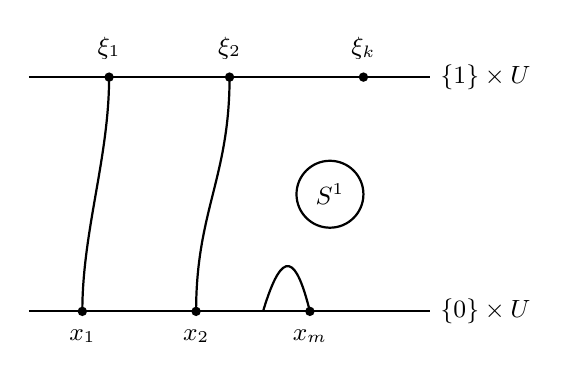
\begin{tikzpicture}[scale=0.85, every node/.style={font=\small}]
  \draw[thick] (0,3.5) -- (6,3.5) node[right] {$\{1\}\times U$};
  \foreach \x/\lab in {1.2/\xi_1, 3/\xi_2, 5/\xi_k}
    \fill (\x,3.5) circle (2pt) node[above=3pt] {$\lab$};
  \draw[thick] (0,0) -- (6,0) node[right] {$\{0\}\times U$};
  \foreach \x/\lab in {0.8/x_1, 2.5/x_2, 4.2/x_m}
    \fill (\x,0) circle (2pt) node[below=3pt] {$\lab$};
  \draw[thick] (0.8,0) .. controls (0.8,1.2) and (1.2,2.3) .. (1.2,3.5);
  \draw[thick] (2.5,0) .. controls (2.5,1.5) and (3,2) .. (3,3.5);
  \draw[thick] (4.5,1.75) circle (0.5) node {$S^1$};
  \draw[thick] (4.2,0) .. controls (4,0.8) and (3.8,1) .. (3.5,0);
\end{tikzpicture}
\par
图 A7.1
\end{minipage}

若一个分支的边界属于同一个面，则由\trOrientation{}的关系，对应的解对\trDegree{}没有贡献；此外，圆周不与边界相交，因而也不贡献。连接不同面的闭区间确实有贡献，而且由\trOrientation{}的关系，贡献量相同。因此
\[\sum_{x\in g_0^{-1}(y)}\operatorname{sign}\det g_0'(x)=\sum_{\xi\in g_1^{-1}(y)}\operatorname{sign}\det g_1'(\xi)\,.\]
我们在此不展开该论证的细节，读者可参考 H.~\trAmann{} [5] 或 J.~\trMilnor{} [157]。我们将通过同调理论以代数方法证明\trDegree{}的存在性。

为了定义容许三元组 $(f,\,U,\,y)$ 的\trDegree{}，我们回忆 $U\subset\R^n$ 是开有界集，$f:\bar{U}\to\R^n$ 连续且 $y\notin f(\partial U)$。将球面 $S^n$ 视为 $\R^n$ 的一点紧化，即 $S^n=\R^n\cup\{\infty\}$，我们现在把 $f$ 视为定义在 $\bar{U}\subset S^n$ 上的球面连续\trMapping{}。记 $U^c=S^n\setminus U$ 为 $U$ 在 $S^n$ 中的补集。注意到 $S^n\setminus\{y\}$ 同胚于 $\R^n$（例如通过球极投影），我们考虑交换图

\noindent\begin{minipage}{\linewidth}
\centering
\begin{tikzpicture}[
  every node/.style={font=\small},
  >->,>=stealth,
  font=\small
]
  \node (A) at (0,0) {$U^{c}\supset\partial U$};
  \node (B) at (5.4,0) {$S^{n}\setminus\{y\}$};
  \node (C) at (5.4,-2.4) {$\R^{n}$};
  \draw[->] (A) -- node[above] {$f|_{\partial U}$} (B);
  \draw[->] (A) -- node[below left,pos=0.55] {$s\circ(f|_{\partial U})$} (C);
  \draw[->] (B) -- node[left] {$s$} node[right] {$\cong$} (C);
\end{tikzpicture}
\par
\end{minipage}

由 Tietze 延拓定理，我们可以将\trMapping{} $s\circ(f|_{\partial U})$ 延拓为连续\trMapping{} $\tilde{f}:U^c\to\R^n$。由于 $\R^n$ 是凸的，所有此类延拓都是\trHomotopic。现在通过 $\tilde{F}:=s^{-1}\circ\tilde{f}:U^c\to S^n\setminus\{y\}$ 定义 $f|_{\partial U}$ 的连续延拓 $\tilde{F}$。则 $f|_{\partial U}$ 的任意两个此类延拓在固定边界值下是\trHomotopic。最后，我们通过
\[F(x):=\begin{cases}f(x) & x\in U\\\tilde{F}(x) & x\in U^c\end{cases}\]
定义扩展 $f:\bar{U}\subset S^n\to S^n$ 的连续\trMapping{} $F:S^n\to S^n$。$F$ 的\trHomotopy{}类不依赖于构造中的选取。考虑 $S^{n}$ 的整数系数同调。我们知道 $H_n(S^n)=\Z$。取 $H_n(S^n)$ 的任意生成元，设为 $o_{S^n}$。则存在整数 $d(F)\in\Z$，定义为
\[F_*\,o_{S^n}=d(F)\,o_{S^n}\,.\]
该整数就是 $F:S^n\to S^n$ 的同调\trDegree{}，我们现在定义
\[d(f,\,U,\,y):=d(F)\in\Z\,.\]
由于 $F$ 的\trHomotopy{}类只依赖于 $(f,\,U,\,y)$ 而不依赖于构造中的选取，该整数是良定义的。我们将利用同调理论验证 $d(f,\,U,\,y)$ 满足公理 1--6。

\textbf{公理 1：}假设 $d(f,\,U,\,y)\neq 0$。则 $F$ 是\trSurjective{}的，因为否则其像将落在一个同胚于 $\R^n$ 的子集中；从而 $F$ 将\trHomotopic{}于常值\trMapping{}，于是 $d(F)=0$。由构造，$y\notin F(U^c)$，因此 $y\in F(U)=f(U)$，蕴含公理 1。

\textbf{公理 2：}与 $(f,\,U,\,y)$ 关联的 $F$ 和与 $(f-y,\,U,\,0)$ 关联的 $G$ 是\trHomotopic，由同调的\trHomotopy\trInvariance{}公理蕴含公理 2。

\textbf{公理 3：}若 $F$ 属于 $(f,\,U,\,y)$，则 $F|_{V}=f|_{V}$ 且 $y\notin F(V^c)$\footnote{原书印作「$y\in F(V^c)$」，其「$\in$」系「$\notin$」之误排——正如上文公理 1 之 $y\notin F(U^c)$，此处唯 $y\notin F(V^c)$ 方与切除公理相容（页图 p-312 取证），径改。——译者注}，蕴含公理 3。

\textbf{公理 6：}对于三元组 $(\mathrm{Id},\,B_1^n(0),\,0)$\footnote{原书印作「$(\mathrm{Id},\,B^{2n}(1),\,0)$」，系「$(\mathrm{Id},\,B_1^n(0),\,0)$」之误排——公理 6 之规范化原用 $d(\mathrm{Id},\,B_1^n(0),\,0)=1$（页图 p-312 取证），径改。——译者注}，我们可以取 $F=\mathrm{Id}:S^n\to S^n$，从而得出 $d(\mathrm{Id}_{S^n})=1$，如所愿。

\textbf{公理 5：}设 $(f_t,\,U,\,y)$，$0\leq t\leq 1$ 是一个容许\trHomotopy。则我们可以构造一个依赖于 $t$ 连续变化的族 $F_t$。因此由同调的\trHomotopy\trInvariance{}，$t\mapsto d(F_t)$ 是常数，蕴含所求。

特别地，我们得出 $d(f,\,U,\,y)$ 仅依赖于 $f|_{\partial U}$。事实上，若 $f:\bar{U}\to\R^n$ 与 $g:\bar{U}\to\R^n$ 在边界上一致：$f|_{\partial U}=g|_{\partial U}$，则 $tf(x)+(1-t)g(x)$，$0\leq t\leq 1$ 定义了一个容许\trHomotopy{}，蕴含 $d(f,\,U,\,y)=d(g,\,U,\,y)$。

\textbf{公理 4：}首先考虑任意的容许三元组 $(f,\,U,\,y)$ 及其在 $S^n$ 上的关联\trMapping{} $F$。假设 $n>0$ 并简记 $S=S^n$，我们有如下交换图：

\noindent\begin{minipage}{\linewidth}
\centering
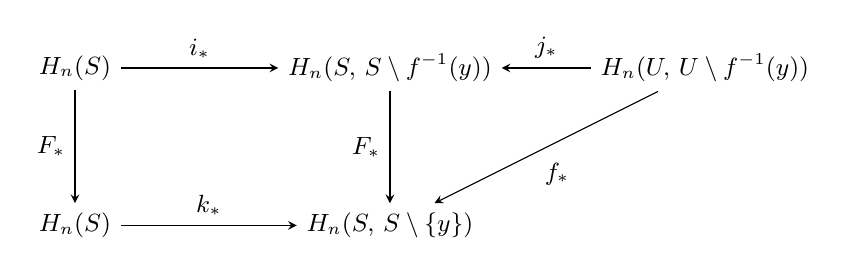
\begin{tikzpicture}[
  node distance=1.6cm and 2.2cm,
  every node/.style={font=\small},
  >->,>=stealth,
  font=\small
]
  \node (A) at (0,2) {$H_n(S)$};
  \node (B) at (4,2) {$H_n(S,\,S\setminus f^{-1}(y))$};
  \node (C) at (8,2) {$H_n(U,\,U\setminus f^{-1}(y))$};
  \node (D) at (0,0) {$H_n(S)$};
  \node (E) at (4,0) {$H_n(S,\,S\setminus\{y\})$};
  \draw[->] (A) -- node[above] {$i_*$} (B);
  \draw[<-] (B) -- node[above] {$j_*$} (C);
  \draw[->] (A) -- node[left] {$F_*$} (D);
  \draw[->] (B) -- node[left] {$F_*$} (E);
  \draw[->] (C) -- node[below right,pos=0.55] {$f_*$} (E);
  \draw[->] (D) -- node[above] {$k_*$} (E);
\end{tikzpicture}
\par
\end{minipage}

\begin{equation}\label{eq:a49-homological-degree}
F_*\,o_S=k_*^{-1}\,f_*\,j_*^{-1}\,i_*(o_S)\,.
\end{equation}

$j_*$ 与 $k_*$ 是同构：前者由同调的\trExcision{}性质，后者作为对 $(S,\,S\setminus\{y\})$ 的长正合序列的推论。

为了证明公理 4，假设 $U=U_1\cup U_2$ 且 $\bar{U}_1\cap\bar{U}_2=\emptyset$，使得 $f_j=f|_{\bar{U}_j}$（$j=1,\,2$）给出容许三元组 $(f_j,\,U_j,\,y)$。我们需要证明
\[d(f,\,U,\,y)=d(f_1,\,U_1,\,y)+d(f_2,\,U_2,\,y)\,.\]
我们将证明

\begin{equation}\label{eq:a50-additivity-decomposition}
f_*\,j_*^{-1}\,i_*(o_S)=f_{1*}\,j_{1*}^{-1}\,i_{1*}(o_S)+f_{2*}\,j_{2*}^{-1}\,i_{2*}(o_S)\,.
\end{equation}

由 (A.49)，这将蕴含 $d(F)\,o_S=d(F_1)\,o_S+d(F_2)\,o_S$，如所愿。为了证明 (A.50) 我们考虑交换图

\noindent\begin{minipage}{\linewidth}
\centering
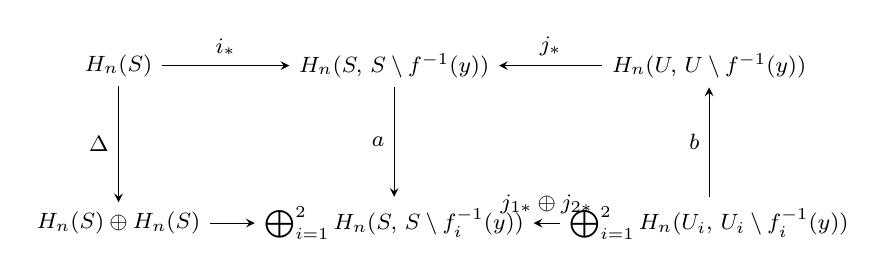
\begin{tikzpicture}[
  node distance=1.4cm and 2cm,
  every node/.style={font=\footnotesize},
  >->,>=stealth,
  font=\footnotesize
]
  \node (A) at (0,2) {$H_n(S)$};
  \node (B) at (3.5,2) {$H_n(S,\,S\setminus f^{-1}(y))$};
  \node (C) at (7.5,2) {$H_n(U,\,U\setminus f^{-1}(y))$};
  \node (D) at (0,0) {$H_n(S)\oplus H_n(S)$};
  \node (E) at (3.5,0) {$\bigoplus_{i=1}^{2}H_n(S,\,S\setminus f_i^{-1}(y))$};
  \node (G) at (7.5,0) {$\bigoplus_{i=1}^{2}H_n(U_i,\,U_i\setminus f_i^{-1}(y))$};
  \draw[->] (A) -- node[above] {$i_*$} (B);
  \draw[<-] (B) -- node[above] {$j_*$} (C);
  \draw[->] (A) -- node[left] {$\Delta$} (D);
  \draw[->] (B) -- node[left] {$a$} (E);
  \draw[<-] (E) -- node[above] {$j_{1*}\oplus j_{2*}$} (G);
  \draw[->] (D) -- (E);
  \draw[<-] (C) -- node[left] {$b$} (G);
\end{tikzpicture}

\bigskip

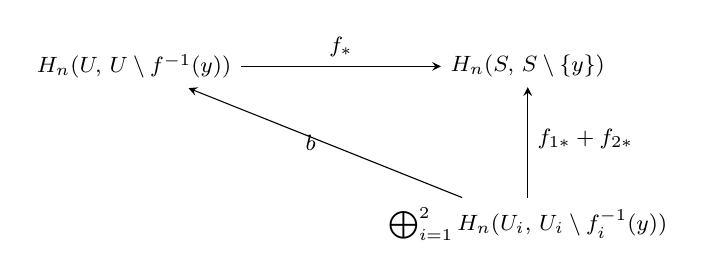
\begin{tikzpicture}[
  node distance=1.6cm and 2.2cm,
  every node/.style={font=\footnotesize},
  >->,>=stealth,
  font=\footnotesize
]
  \node (A) at (0,0) {$H_n(U,\,U\setminus f^{-1}(y))$};
  \node (B) at (5,0) {$H_n(S,\,S\setminus\{y\})$};
  \node (C) at (5,-2) {$\bigoplus_{i=1}^{2}H_n(U_i,\,U_i\setminus f_i^{-1}(y))$};
  \draw[->] (A) -- node[above] {$f_*$} (B);
  \draw[->] (C) -- node[above right,pos=0.35] {$f_{1*}+f_{2*}$} (B);
  \draw[->] (C) -- node[left] {$b$} (A);
\end{tikzpicture}
\par
\end{minipage}

根据同调的\trExcision{}性，\trMapping{} $j_*$ 与 $j_{1*}\oplus j_{2*}$ 是同构。\trMapping{} $\Delta:\beta\mapsto(\beta,\,\beta)$ 是对角\trMapping{}。此外，$a(\sigma)=(a_{1*}(\sigma),\,a_{2*}(\sigma))$ 且 $b(\sigma_1,\,\sigma_2)=b_{1*}(\sigma_1)+b_{2*}(\sigma_2)$，其中 $a_j:(S,\,S\setminus f^{-1}(y))\to(S,\,S\setminus f_j^{-1}(y))$ 且 $b_j:(U_j,\,U_j\setminus f_j^{-1}(y))\to(U,\,U\setminus f^{-1}(y))$。注意到对 $j=1,\,2$ 有 $f\circ b_j=f_j$。若 $\beta\in H_n(S)$，我们可以计算
\begin{align*}
f_*\,j_*^{-1}\,i_*(\beta) &= f_*\,b\,(j_{1*}\oplus j_{2*})^{-1}\,(i_{1*}\oplus i_{2*})\circ\Delta(\beta) \\&= f_*\bigl(b_{1*}\,j_{1*}^{-1}\,i_{1*}(\beta)+b_{2*}\,j_{2*}^{-1}\,i_{2*}(\beta)\bigr) \\
&= f_{1*}\,j_{1*}^{-1}\,i_{1*}(\beta)+f_{2*}\,j_{2*}^{-1}\,i_{2*}(\beta)\,,
\end{align*}
正如 (A.50) 所声称的。我们验证了公理 4 成立。综上所述，我们证明了 $d$ 满足全部公理，因此\trMapping\trDegree{}的存在性证明到此完成。

\trhRemark：\trBrouwer\trDegree{}可以推广到任意的赋范向量空间 $E$，不过仅限于一类受限的连续\trMapping{}。我们称三元组 $(f,\,\Omega,\,y)$ 为\textbf{容许的}，若 $\Omega\subset E$ 是有界开子集，$f:\bar{\Omega}\to E$ 是形如 $f=\mathrm{id}-k$（$k$ 为\trCompact{}\trMapping{}，即 $k(\bar{\Omega})$ 的闭包在 $E$ 中是\trCompact{}的）的连续\trMapping{}，且 $y\in E$ 满足 $y\notin f(\partial\Omega)$。存在唯一的\trMapping{}将每个容许三元组关联到一个整数 $d(f,\,\Omega,\,y)\in\Z$ 且满足公理 1--6。它被称为\trLeray-\trSchauder\trDegree；我们在第 3 章中使用了该\trDegree{}以建立\trSymplecticCapacity{} $c_0$ 的存在性。构造此推广的关键观察是，\trCompact{}\trMapping{}可以在（一致拓扑下）被其像落在 $E$ 的有限维\trSubspace{}中的\trCompact{}\trMapping{}逼近。取这样的\trMapping{} $k$ 满足 $k(\bar{\Omega})\subset E_n\subset E$，其中 $\dim E_n=n$。若 $x\in E$ 是
$(\mathrm{id}-k)(x)=0$
的解，则 $x\in E_n$，因而我们定义
\[d(\mathrm{id}-k,\,\Omega,\,0)=d(\mathrm{id}-k,\,\Omega\cap E_n,\,0)\,,\]
其中右端是\trBrouwer\trDegree。该定义是良定义的。事实上，若选取更大的有限维空间 $E_m\supset E_n$，则 $d(\mathrm{id}-k,\,\Omega\cap E_n,\,0)=d(\mathrm{id}-k,\,\Omega\cap E_m,\,0)$。这可以通过用具有 $0$ 作为\trRegular{}值的\trSmooth{}\trMapping{}逼近 $(\mathrm{id}-k)|_{\Omega\cap E_m}$ 并利用
\cref{prop:brouwer-degree-formula}(i)\footnote{原书引作「Proposition 1」，编号有误，实指本节命题 7，此处径改实标。——译者注} 计算指标来证明。由于有限维\trMapping{}在\trCompact{}\trMapping{}集合中（在一致拓扑下）是\trDense{}的，上面定义的连续\trMapping{} $(\mathrm{id}-k,\,\Omega,\,0)\mapsto d(\mathrm{id}-k,\,\Omega,\,0)\in\Z$ 具有唯一延拓，称为\trLeray-\trSchauder\trDegree。细节请读者参考 H.~\trAmann{} [5]、K.~\trDeimling{} [60] 与 E.~\trZeidler{} [232] 第 12 章。